% ===== handout mode =====
% Comment/uncomment this line to toggle handout mode
% \newcommand{\handout}{}

% Comment/uncoment this line to toogle Mortitz mode
% \newcommand{\Moritz}{}

% Comment/uncomment this line to toggle handout mode
% \newcommand{\handout}{}

% by Stephan

%% Moritz mode or Stephan mode
\ifdefined \MoritzMode

% This is a configuration file with private, tutor specific information.
% It is therefore excluded from the Git repository so changes in this file will not conflict in git commits.

% Copy this Template, rename to config.tex and add your information below.

\newcommand{\mymail}{moritz.laupichler@student.kit.edu} % Consider using your named student Mail address to keep your u-Account private.

\newcommand{\myname}{\href{mailto:\mymail}{Moritz Laupichler}}

\newcommand{\mytutnumber}{27}

\newcommand{\mytutinfos}{Dienstags, 5. Block (15:45-17:15), SR 236}

\newcommand{\aboutMeFrame}{
	\begin{frame}{Euer Tutor}
		Name: \myname \\
		Alter: 19 Jahre \\
		Studiengang: Bachelor Informatik, 3. Semester \\
		\vspace{1cm}
		\pause 
		\centering{Kontakt: \href{mailto:\mymail}{\mymail}}
	\end{frame}
}

% Toggle Handout mode by including the following line before including style_tut
% and removing the % at the start (but do NOT remove it here, otherwise handout mode will always be on!)
% Please keep handout mode on in all commits!

% \newcommand{\handout}{} % Moritz mode
\fi
\ifdefined \AlexMode

% This is a configuration file with private, tutor specific information.
% It is therefore excluded from the Git repository so changes in this file will not conflict in git commits.

% Copy this Template, rename to config.tex and add your information below.

\newcommand{\mymail}{alexander.klug@student.kit.edu} % Consider using your named student Mail address to keep your u-Account private.

\newcommand{\myname}{\href{mailto:\mymail}{Alexander Klug}}

\newcommand{\mytutnumber}{30}

\newcommand{\mytutinfos}{Mittwochs, 3. Block (11:30-13:00), SR -107}

\newcommand{\aboutMeFrame}{
	\begin{frame}{Euer Tutor}
		Name: \myname \\
		Alter: 19 Jahre \\
		Studiengang: Bachelor Informatik, 3. Semester \\
		\vspace{1cm}
		\pause 
		\centering{Kontakt: \href{mailto:\mymail}{\mymail}}
	\end{frame}
}

% Toggle Handout mode by including the following line before including style_tut
% and removing the % at the start (but do NOT remove it here, otherwise handout mode will always be on!)
% Please keep handout mode on in all commits!

% \newcommand{\handout}{} % Alex Mode
\fi
\ifdefined \StephanMode

% This is a configuration file with private, tutor specific information.
% It is therefore excluded from the Git repository so changes in this file will not conflict in git commits.

% Copy this Template, rename to config.tex and add your information below.

\newcommand{\mymail}{stephan.bohr@student.kit.edu} % Consider using your named student Mail address to keep your u-Account private.

\newcommand{\myname}{\href{mailto:\mymail}{Stephan Bohr}}

\newcommand{\mytutnumber}{19}

\newcommand{\mytutinfos}{Dienstags, 3. Block (11:30-13:00), SR -108}

\newcommand{\aboutMeFrame}{
	\begin{frame}{Euer Tutor}
		Name: \myname \\
		Alter: 21 Jahre \\
		Studiengang: Bachelor Informatik, 5. Semester \\
		\vspace{1cm}
		\pause 
		\centering{Kontakt: \href{mailto:\mymail}{\mymail}}
	\end{frame}
} % Stephan mode
\fi

%% Beamer-Klasse im korrekten Modus
\ifdefined \handout
\documentclass[handout]{beamer} % Handout mode
\else
\documentclass{beamer}
\fi
%\documentclass[18pt,parskip]{beamer}

%% SLIDE FORMAT

% use 'beamerthemekit' for standard 4:3 ratio
% for widescreen slides (16:9), use 'beamerthemekitwide'

\usepackage{../templates/KIT-slides/beamerthemekit}
%\usepackage{../templates/KIT-slides/beamerthemekitwide}

%% TITLE PICTURE

% if a custom picture is to be used on the title page, copy it into the 'logos'
% directory, in the line below, replace 'mypicture' with the 
% filename (without extension) and uncomment the following line
% (picture proportions: 63 : 20 for standard, 169 : 40 for wide
% *.eps format if you use latex+dvips+ps2pdf, 
% *.jpg/*.png/*.pdf if you use pdflatex)

\titleimage{../figures/titleimage/brain}

%% TITLE LOGO

% for a custom logo on the front page, copy your file into the 'logos'
% directory, insert the filename in the line below and uncomment it

%\titlelogo{mylogo}

% (*.eps format if you use latex+dvips+ps2pdf,
% *.jpg/*.png/*.pdf if you use pdflatex)

%% TikZ INTEGRATION

% use these packages for PCM symbols and UML classes
% \usepackage{templates/tikzkit}
% \usepackage{templates/tikzuml}

%\usepackage{tikz}
%\usetikzlibrary{matrix}
%\usetikzlibrary{arrows.meta}
%\usetikzlibrary{automata}
%\usetikzlibrary{tikzmark}

%%%%%%%%%%%%%%%%%%%%%%%%%
% Libertine font (Original GBI font)
\usepackage[mono=false]{libertine}
%\renewcommand*\familydefault{\sfdefault}  %% Only if the base font of the document is to be sans serif

%% Schönere Schriften
\usepackage[TS1,T1]{fontenc}

%% Deutsche Silbentrennung und Beschriftungen
\usepackage[ngerman]{babel}

%% UTF-8-Encoding
\usepackage[utf8]{inputenc}

%% Bibliotheken für viele mathematische Symbole
\usepackage{amsmath, amsfonts, amssymb}

%% Anzeigetiefe für Inhaltsverzeichnis: 1 Stufe
\setcounter{tocdepth}{1}

%% Hyperlinks
\usepackage{hyperref}
% I don't know why, but this works and only includes sections and NOT subsections in the pdf-bookmarks.
\hypersetup{bookmarksdepth=subsection}

%% remove navigation symbols
\setbeamertemplate{navigation symbols}{}

%% switch between "ngerman" and "english" for German/English style date and logos
\selectlanguage{ngerman}

%% for invisible pause texts instead of dimming
\setbeamercovered{invisible}

\usepackage[german=swiss]{csquotes}

\usepackage{tabularx}
\usepackage{booktabs}

\usepackage{tikz}


% Problem: disabled itemize-icons
%\usepackage{enumitem}
% %\setlist[enumerate]{topsep=0pt,itemsep=-1ex,partopsep=1ex,parsep=1ex}
% \setlist[itemize]{noitemsep, nolistsep}
% \setlist[enumerate]{noitemsep, nolistsep}

% Mathmode no vertical space (https://tex.stackexchange.com/a/47403/146825)
\setlength{\abovedisplayskip}{0pt}
\setlength{\belowdisplayskip}{0pt}
\setlength{\abovedisplayshortskip}{0pt}
\setlength{\belowdisplayshortskip}{0pt}

%%%%%%%%%%%% Slides %%%%%%%%%%%%%%%%

\newcommand{\Moritz}[1]{
	\ifdefined \MoritzMode
	#1
	\fi
}

\newcommand{\Alex}[1]{
	\ifdefined \AlexMode
	#1
	\fi
}

\newcommand{\Stephan}[1]{
	\ifdefined \StephanMode
	#1
	\fi
}

\newcommand{\notMoritz}[1]{
	\Alex{#1} \Stephan{#1}
}

\newcommand{\notAlex}[1]{
	\Moritz{#1} \Stephan{#1}
}

\newcommand{\notStephan}[1]{
	\Alex{#1} \Moritz{#1}
}

%% Wochennummer
%\newcounter{weeknum}

%% Titelinformationen
%\title[GBI Tutorium, Woche \theweeknum]{Grundbegriffe der Informatik \\ Tutorium \mytutnumber}
%\subtitle{Termin \theweeknum \ | \mydate \\ \myname}
\author[\myname]{\myname}
\institute{Fakultät für Informatik}
%\date{\mydate}

%% Titel einfügen
\newcommand{\titleframe}{\frame{\titlepage}\addtocounter{framenumber}{-1}}


%% Alles starten mit \starttut{X}
%\newcommand{\starttut}[1]{\setcounter{weeknum}{#1}\titleframe\frame{\frametitle{Inhalt}\tableofcontents} \AtBeginSection[]{%
%\begin{frame}
%	\tableofcontents[currentsection]
%\end{frame}\addtocounter{framenumber}{-1}}}


%\newcommand{\framePrevEpisode}{
%	\begin{frame}
%		\centering
%		\textbf{In the previous episode of GBI...}
%	\end{frame}
%}

%% Roadmap frame
%table of contents
\newcommand{\roadmap}{
	\frame{\frametitle{Roadmap}\tableofcontents}}

 \AtBeginSection[]{%
\begin{frame}
	\frametitle{Roadmap}
	\tableofcontents[currentsection]
\end{frame}%\addtocounter{framenumber}{-1}
}


%% ShowMessage frame
\newcommand{\showmessage}[1]{\frame{\frametitle{\phantom{1em}}\centering\textbf{#1}}}

%% Fragen
%% Lastframe
\newcommand{\questionframe}{\showmessage{Fragen?}}

%% Lastframe
\newcommand{\lastframe}{\showmessage{Vielen Dank für Eure Aufmerksamkeit! \\Bis nächste Woche :)}}

%% Thanks frame
\newcommand{\slideThanks}{
	\begin{frame}
		\frametitle{Credits}
		\begin{block}{}
			An der Erstellung des Foliensatzes haben mitgewirkt:\\[1em]
			\Moritz{
			Stephan Bohr \\
			Alexander Klug \\
			}
			\Alex{
			Stephan Bohr \\
			Moritz Laupichler \\
			}
			\Stephan{
			Moritz Laupichler \\
			Alexander Klug \\
			}
			Katharina Wurz \\
			Thassilo Helmold \\
			Daniel Jungkind \\
			% Philipp Basler \\
			% Nils Braun \\
			% Dominik Doerner \\
			% Ou Yue \\
		\end{block}
	\end{frame}
}

%% Verbatim
%\usepackage{moreverb}

% GBI related stuff, but not beamer-stuff
\newcommand{\newpar}[1]{\paragraph{#1}\mbox{}\newline}

\newcommand{\nM}{\mathbb{M}}
\newcommand{\nR}{\mathbb{R}}
\newcommand{\nN}{\mathbb{N}}
\newcommand{\nZ}{\mathbb{Z}}
\newcommand{\nQ}{\mathbb{Q}}
\newcommand{\nB}{\mathbb{B}}
\newcommand{\nC}{\mathbb{C}}
\newcommand{\nK}{\mathbb{K}}
\newcommand{\nF}{\mathbb{F}}
\newcommand{\nG}{\mathbb{G}}
\newcommand{\nullel}{\mathcal{O}}
\newcommand{\einsel}{\mathds{1}}
\newcommand{\nP}{\mathbb{P}}
\newcommand{\Pot}{\mathcal{P}}
\renewcommand{\O}{\text{O}}

\newcommand{\bfmod}{\ensuremath{\text{\textbf{ mod }}}}
\renewcommand{\mod}{\bfmod}
\newcommand{\bfdiv}{\ensuremath{\text{\textbf{ div }}}}
\renewcommand{\div}{\bfdiv}


\newcommand{\set}[1]{\left\{ #1 \right\}}
\newcommand{\setc}[2]{\set{#1 \mid #2}}
\newcommand{\setC}[2]{\set{#1 \mid \text{ #2 }}}

\newcommand{\setsize}[1]{\; \mid #1 \mid \; }

\newcommand{\q}[1]{\textquotedblleft #1\textquotedblright}

% Zu zeigen, thx to http://www.matheboard.de/archive/155832/thread.html
\newcommand{\zz}{\ensuremath{\mathrm{z\kern-.29em\raise-0.44ex\hbox{z}}}:}

% Text above symbol
% https://tex.stackexchange.com/a/74132/146825
%
% \newcommand{\eqtext}[1]{\stackrel{\mathclap{\normalfont\mbox{#1}}}{=}}
% \newcommand{\gdwtext}[1]{\stackrel{\mathclap{\normalfont\mbox{#1}}}{\Leftrightarrow}}
% \newcommand{\imptext}[1]{\stackrel{\mathclap{\normalfont\mbox{#1}}}{\Rightarrow}}
% \newcommand{\symbtext}[2]{\stackrel{\mathclap{\normalfont\mbox{#2}}}{#1}}
\newcommand{\eqtext}[1]{\mathrel{\overset{\makebox%[0pt]
{\mbox{\normalfont\tiny #1}}}{=}}}
\newcommand{\gdwtext}[1]{\mathrel{\overset{\makebox%[0pt]
{\mbox{\normalfont\tiny #1}}}{\ensuremath{\Leftrightarrow}}}}
\newcommand{\imptext}[1]{\mathrel{\overset{\makebox%[0pt]
{\mbox{\normalfont\tiny #1}}}{\ensuremath{\Rightarrow}}}}
\newcommand{\symbtext}[2]{\mathrel{\overset{\makebox%[0pt]
{\mbox{\normalfont\tiny #2}}}{#1}}}

% qed symbol
\newcommand{\qedblack}{\hfill \ensuremath{\blacksquare}}
\newcommand{\qedwhite}{\hfill \ensuremath{\Box}}

% Aussagenlogik
% Worsch
\colorlet{alcolor}{blue}
\RequirePackage{tikz}
\usetikzlibrary{arrows.meta}
\newcommand{\alimpl}{\mathrel{\tikz[x={(0.1ex,0ex)},y={(0ex,0.1ex)},>={Classical TikZ Rightarrow[]}]{\draw[alcolor,->,line width=0.7pt,line cap=round] (0,0) -- (15,0);\path (0,-6);}}}
\newcommand{\alimp}{\alimpl}
\newcommand{\aleqv}{\mathrel{\tikz[x={(0.1ex,0ex)},y={(0ex,0.1ex)},>={Classical TikZ Rightarrow[]}]{\draw[alcolor,<->,line width=0.7pt,line cap=round] (0,0) -- (18,0);\path (0,-6);}}}
\newcommand{\aland}{\mathbin{\raisebox{-0.6pt}{\rotatebox{90}{\texttt{\color{alcolor}\char62}}}}}
\newcommand{\alor}{\mathbin{\raisebox{-0.8pt}{\rotatebox{90}{\texttt{\color{alcolor}\char60}}}}}
%\newcommand{\ali}[1]{_{\mathtt{\color{alcolor}#1}}}
\newcommand{\alv}[1]{\mathtt{\color{alcolor}#1}}
\newcommand{\alnot}{\mathop{\tikz[x={(0.1ex,0ex)},y={(0ex,0.1ex)}]{\draw[alcolor,line width=0.7pt,line cap=round,line join=round] (0,0) -- (10,0) -- (10,-4);\path (0,-8) ;}}}
\newcommand{\alP}{\alv{P}} %ali{#1}}
%\newcommand{\alka}{\negthinspace\hbox{\texttt{\color{alcolor}(}}}
\newcommand{\alka}{\negthinspace\text{\texttt{\color{alcolor}(}}}
%\newcommand{\alkz}{\texttt{\color{alcolor})}}\negthinspace}
\newcommand{\alkz}{\text{\texttt{\color{alcolor})}}\negthinspace}

% Thassilo
\newcommand{\BB}{\mathbb{B}}
\newcommand{\boder}{\alor}%{\ensuremath{\text{\;}\textcolor{blue}{\vee}}\text{\;}}
\newcommand{\bund}{\aland}%{\ensuremath{\text{\;}\textcolor{blue}{\wedge}}\text{\;}}
\newcommand{\bimp}{\alimp}%{\ensuremath{\text{\;}\textcolor{blue}{\to}}\text{\;}}
\newcommand{\bnot}{\alnot}%{\ensuremath{\text{\;}\textcolor{blue}{\neg}}\text{}}
\newcommand{\bgdw}{\aleqv}%{\ensuremath{\text{\;}\textcolor{blue}{\leftrightarrow}}\text{\;}}
\newcommand{\bone}{\ensuremath{\textcolor{blue}{1}}\text{}}
\newcommand{\bzero}{\ensuremath{\textcolor{blue}{0}}\text{}}
\newcommand{\bleftBr}{\alka}%{\ensuremath{\textcolor{blue}{(}}\text{}}
\newcommand{\brightBr}{\alkz}%{\ensuremath{\textcolor{blue}{)}}\text{}}

\newcommand{\val}{\hbox{\textit{val}}}

\newcommand{\VarAL}{\hbox{\textit{Var}}_{AL}}
\newcommand{\ForAL}{\hbox{\textit{For}}_{AL}}

% Validierungsfunktion val_i
\newcommand{\vali}[1]{\ensuremath{\val_I(#1)}}

% Boolsche Funktion b_
\newcommand{\bfnot}[1]{\ensuremath{b_{\bnot}(#1)}}
\newcommand{\bfand}[2]{\ensuremath{b_{\bund}(#1,#2)}}
\newcommand{\bfor}[2]{\ensuremath{b_{\boder}(#1,#2)}}
\newcommand{\bfimp}[2]{\ensuremath{b_{\bimp}(#1,#2)}}

% Aussagenkalkül
\newcommand{\AAL}{A_{AL}}
\newcommand{\LAL}{\hbox{\textit{For}}_{AL}}
\newcommand{\AxAL}{\hbox{\textit{Ax}}_{AL}}
\newcommand{\MP}{\hbox{\textit{MP}}}

% Prädikatenlogik
% die nachfolgenden Sachen angepasst an cmtt
\newlength{\ttquantwd}
\setlength{\ttquantwd}{1ex}
\newlength{\ttquantht}
\setlength{\ttquantht}{6.75pt}
\def\plall{%
  \tikz[line width=0.67pt,line cap=round,line join=round,baseline=(B),alcolor] {
    \draw (-0.5\ttquantwd,\ttquantht) -- node[coordinate,pos=0.4] (lll){} (-0.25pt,-0.0pt) -- (0.25pt,-0.0pt) -- node[coordinate,pos=0.6] (rrr){} (0.5\ttquantwd,\ttquantht);
    \draw (lll) -- (rrr);
    \coordinate (B) at (0,-0.35pt);
  }%
}
\def\plexist{%
  \tikz[line width=0.67pt,line cap=round,line join=round,baseline=(B),alcolor] {
    \draw (-0.9\ttquantwd,\ttquantht) -- (0,\ttquantht) -- node[coordinate,pos=0.5] (mmm){} (0,0) --  (-0.9\ttquantwd,0);
    \draw (mmm) -- ++(-0.75\ttquantwd,0);
    \coordinate (B) at (0,-0.35pt);
  }\ensuremath{\,}%
}
\let\plexists=\plexist
\newcommand{\NT}[1]{\ensuremath{\langle\mathrm{#1} \rangle}}
\newcommand{\CPL}{\text{\itshape Const}_{PL}}
\newcommand{\FPL}{\text{\itshape Fun}_{PL}}
\newcommand{\RPL}{\text{\itshape Rel}_{PL}}
\newcommand{\VPL}{\text{\itshape Var}_{PL}}
\newcommand{\plka}{\alka}
\newcommand{\plkz}{\alkz}
%\newcommand{\plka}{\plfoo{(}}
%\newcommand{\plkz}{\plfoo{)}}
\newcommand{\plcomma}{\hbox{\texttt{\color{alcolor},}}}
\newcommand{\pleq}{{\color{alcolor}\,\dot=\,}}

\newcommand{\plfoo}[1]{\mathtt{\color{alcolor}#1}}
\newcommand{\plc}{\plfoo{c}}
\newcommand{\pld}{\plfoo{d}}
\newcommand{\plf}{\plfoo{f}}
\newcommand{\plg}{\plfoo{g}}
\newcommand{\plh}{\plfoo{h}}
\newcommand{\plx}{\plfoo{x}}
\newcommand{\ply}{\plfoo{y}}
\newcommand{\plz}{\plfoo{z}}
\newcommand{\plR}{\plfoo{R}}
\newcommand{\plS}{\plfoo{S}}
\newcommand{\ar}{\mathrm{ar}}

\newcommand{\bv}{\mathrm{bv}}
\newcommand{\fv}{\mathrm{fv}}

\def\word#1{\hbox{\textcolor{blue}{\texttt{#1}}}}
%\let\literal\word
\def\mword#1{\hbox{\textcolor{blue}{$\mathtt{#1}$}}}  % math word
\def\sp{\scalebox{1}[.5]{\textvisiblespace}}
\def\wordsp{\word{\sp}}


\newcommand{\W}{\ensuremath{\hbox{\textbf{w}}}\xspace}
\newcommand{\F}{\ensuremath{\hbox{\textbf{f}}}\xspace}
\newcommand{\WF}{\ensuremath{\{\W,\F\}}\xspace}
\newcommand{\valDIb}{\val_{D,I,\beta}}

\newcommand{\impl}{\ifmmode\ensuremath{\mskip\thinmuskip\Rightarrow\mskip\thinmuskip}\else$\Rightarrow$\fi\xspace}
\newcommand{\Impl}{\ifmmode\implies\else$\Longrightarrow$\fi\xspace}

\newcommand{\derives}{\Rightarrow}

\newcommand{\gdw}{\ifmmode\mskip\thickmuskip\Leftrightarrow\mskip\thickmuskip\else$\Leftrightarrow$\fi\xspace}
\newcommand{\Gdw}{\ifmmode\iff\else$\Longleftrightarrow$\fi\xspace}

\newcommand*{\from}{\colon}
\newcommand{\functionto}{\longrightarrow}


\newcommand{\LTer}{L_{\text{\itshape Ter}}}
\newcommand{\LRel}{L_{\text{\itshape Rel}}}
\newcommand{\LFor}{L_{\text{\itshape For}}}
\newcommand{\NTer}{N_{\text{\itshape Ter}}}
\newcommand{\NRel}{N_{\text{\itshape Rel}}}
\newcommand{\NFor}{N_{\text{\itshape For}}}
\newcommand{\PTer}{P_{\text{\itshape Ter}}}
\newcommand{\PRel}{P_{\text{\itshape Rel}}}
\newcommand{\PFor}{P_{\text{\itshape For}}}

\newcommand{\sgn}{\mathop{\text{sgn}}}

\newcommand{\lang}[1]{\ensuremath{\langle#1\rangle}}

\newcommand{\literal}[1]{\hbox{\textcolor{blue!95!white}{\textup{\texttt{\scalebox{1.11}{#1}}}}}}
\let\hashtag\#
\renewcommand{\#}[1]{\literal{#1}}

\def\blank{\ensuremath{\openbox}}
\def\9{\blank}
\newcommand{\io}{\!\mid\!}


\providecommand{\fspace}{\mathord{\text{space}}}
\providecommand{\fSpace}{\mathord{\text{Space}}}
\providecommand{\ftime}{\mathord{\text{time}}}
\providecommand{\fTime}{\mathord{\text{Time}}}

\newcommand{\fnum}{\text{num}}
\newcommand{\fNum}{{\text{Num}}}

\def\Pclass{\text{\bfseries P}}
\def\PSPACE{\text{\bfseries PSPACE}}



\title[Komplexität, Entscheidbarkeit, reguläre Sprachen]{13. Tutorium\\ Komplexität, Entscheidbarkeit, reguläre Sprachen}
\subtitle{Grundbegriffe der Informatik, Tutorium \hashtag \mytutnumber}
\date{\today}


\usetikzlibrary{matrix}
\usetikzlibrary{arrows.meta}
\usetikzlibrary{automata}
\usetikzlibrary{tikzmark}

\begin{document}
\titleframe
\begin{frame}{Organisatorisches}
	\begin{itemize}
		\item Für \emph{Übungsschein} angemeldet?
		\item Für \emph{Klausur} angemeldet?
		\item 120 Punkte sind hinreichend für den Übungsschein.
		%\Stephan{\item Ab heute liegen alle Übungsblätter \emph{1-12} im Wägelchen.}
	\end{itemize}
\end{frame}

\roadmap

%%%%%%%%%% %%%%%%%%%%

\Moritz{

\section{MIMA-X}
\subsection{Mimax}

\begin{frame}{Struktur}
	\centering
	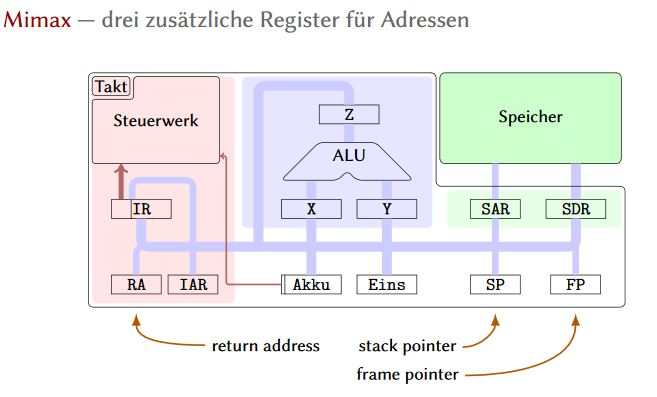
\includegraphics[width=\textwidth]{../topics/mimax/mimax_structure.jpg} 
\end{frame}

\begin{frame}{Neue Befehle}
	\begin{block}{CALL adr}
			\begin{itemize}
				\item ähnlich wie \emph{JMP} adr
				\item zusätzlich wird Inhalt vom IAR ins RA geschrieben
			\end{itemize}
		\end{block}
		
		\begin{block}{RET}
			\begin{itemize}
				\item ähnlich wie \emph{JMP} adr
				\item zusätzlich wird Inhalt vom RA ins IAR geschrieben
			\end{itemize}			
		\end{block}
	\emph{CALL adr} ruft also unsere Subroutine auf und mit \emph{RET} kehren wir von der Subroutine zurück zum Hauptprogramm
	\end{frame}

\begin{frame}{SP und FP}
	\begin{block}{stack pointer}
		zeigt auf Stelle an die \emph{push} den nächsten Wert legen würde\\
		\emph{LDVR disp(SP)} holt oberstes Speicherelement in Akku\\
		\emph{STVR disp(SP)} speichert Akkuinhalt als oberstes Stackelement	
	\end{block}
	\begin{block}{frame pointer}
			funktioniert ähnlich wie SP, genaueres in anderen Vorlesungen
	\end{block}
\end{frame}

\begin{frame}
	Für Beispiele mit der pointer-Magie schaut euch am besten die Vorlesungsfolien an!
\end{frame}

\begin{frame}{Aufgabe}
	\begin{exampleblock}{Aufgabe}
		Schreibe ein Programm, das eine an Adresse $a$ gegebene Zahl mittels einer Subroutine negiert und danach wieder in $a$ speichert. Die Adresse $R$ sei zum Zwischenspeichern frei verfügbar.
	\end{exampleblock}
\end{frame}

\begin{frame}
	\begin{block}{Lösung}
		\emph{main}LDV $a$\\
		CALL sub\\	
		HALT\\
		\emph{sub}:NOT\\
		STV $R$\\
		LDC 1\\
		ADD $R$\\
		STV $a$\\
		RET
	\end{block}
\end{frame}

}

\section{Komplexität und Entscheidbarkeit}
\subsection{Wiederholung Turing-Maschinen}

\begin{frame}[fragile]{Turingmaschinen (Wdh.)}
   \begin{figure}[ht]
  		\centering
  		\begin{tikzpicture}[node distance=0mm,->,>={Latex[open]},thin]
    		\matrix[matrix of math nodes,column sep=0mm,minimum size=8mm,row sep=10mm,nodes={every rectangle node/.style={rectangle,draw,anchor=center}}]   {
      		& & & && \node[circle,draw] (z) {z}; & \\
      		\node[circle] {\cdots}; & \blank & \blank & |(x)| \#a & \#b & \#b & \#a & \#a & \blank & \node[circle] {\cdots};\\
    		};
    		\path[<->] (z) edge [out=270,in=90] (x);
  		\end{tikzpicture}
	\end{figure}
\end{frame}

\begin{frame}{Turingmaschinen (Wdh.)}
	\begin{block}{Def.: Turingmaschine}
		Eine \textbf{Turingmaschine} $T=(Z,z_0,X,f,$ $g,m)$ ist festgelegt durch
			\begin{itemize}
			\item eine \textbf{Zustandsmenge} $Z$
			\item einen \textbf{Anfangszustand} $z_0\in Z$
			\item ein \textbf{Bandalphabet} $X$
			\item eine partielle \textbf{Zustandsüberführungsfunktion} $f:Z\times X \dashrightarrow Z$
			\item eine partielle \textbf{Ausgabefunktion} $g:Z\times X \dashrightarrow X$ und
			\item eine partielle \textbf{Bewegungsfunktion} $m:Z\times X \dashrightarrow \{L, 0, R\}$
			\begin{itemize}
				\item $f$, $g$ und $m$ seien für die gleichen Paare $(z,x)\in Z\times X$ definiert bzw. nicht definiert
			\end{itemize}
			\item[]
			\item TM liest von Band, schreibt auf Band und kann ihren Kopf bewegen
			\end{itemize} 
	\end{block}
\end{frame}

\begin{frame}[fragile]{Turingmaschinen (Wdh.)}
    \begin{columns}\footnotesize
    	\begin{column}{0.4\textwidth}
    		\begin{tikzpicture}[shorten >=1pt,initial text=,node distance=1.7cm,auto,->,>=stealth,baseline=(B.base)]
          		% \node[state,initial]  (S)                       {$S$};
          		\node[state,initial]  (A)          {$A$};
          		% \node (nix) [right of=A] {};
          		\node[state]          (B) [above right of=A] {$B$};
          		\node[state]          (C) [right of=B] {$C$};
          		\node[state]          (E) [below right of=A] {$E$};
          		\node[state]          (D) [right of=E] {$D$};
          		\path[->]
          		% (S) edge              node  {$\9\io\9R$} (A)
          		(A) edge              node  {$\#1\io\#XR$} (B)
          		(B) edge [loop above] node  {$\#1\io\#1R$} ()
          		edge              node  {$\9\io\9R$} (C)
          		(C) edge [loop above] node  {$\#1\io\#1R$} ()
          		edge              node  {$\9\io\#1L$} (D)
          		(D) edge [loop below] node  {$\#1\io\#1L$} ()
          		edge              node  {$\9\io\9L$} (E)
          		(E) edge [loop below] node  {$\#1\io\#1L$} ()
          		edge              node  {$\#X\io\#1R$} (A)
          		% (B) edge              node        {$\9\io\9R$} (B)
          		% edge [loop right] node        {$\#1\io\#1R$} ()
          		% (B) edge [loop right] node {$\9\io\#1L$} ()
          		% edge  node [pos=0.3]       {$\#1\io\#1L$} (A)
          		;
        \end{tikzpicture}
		\end{column}
		\begin{column}{0.6\textwidth}
			\begin{tabular}[t]{>{$}c<{$}@{\quad}*{6}{>{$}c<{$}}}
          		\toprule
          		& A       & B      & C       & D       & E \\
          		\midrule
          		\9       
          		&         & \9,R,C & \#1,L,D & \9,L,E  &  \\
          		\#1         & \#X,R,B & \#1,R,B& \#1,R,C & \#1,L,D & \#1,L,E \\
          		\#X         &         &        &         &         & \#1,R,A \\
          		\bottomrule
        	\end{tabular}
        	\normalsize
        	\begin{exampleblock}{Aufgabe}
        		\begin{enumerate}
        			\item Was steht bei der Eingabe von \#{111} auf dem Band?
        			\item Was macht die TM allgemein, wenn man auf der ersten \#1 startet?
        		\end{enumerate}
        	\end{exampleblock}
		\end{column}
	\end{columns}
\end{frame}

\Stephan{
\begin{frame}{Turingmaschinen}
  \begin{exampleblock}{Aufgabe}
     \begin{tabular}[t]{>{$}c<{$}@{\qquad}*{4}{>{$}c<{$}}}
          \toprule
          & r & c_0 & c_1 & h \\
          \midrule
          \#0 & \#0,R,r   & \#0,L,c_0 & \#1,L,c_0 \\
          \#1 & \#1,R,r   & \#1,L,c_0 & \#0,L,c_1 \\
          \9  & \9, L,c_1 & \9 ,R,h   & \#1,L,c_0 & \hphantom{\#1,L,C} \\
          \bottomrule
        \end{tabular}\\[2em]

        $r$ ist der Anfangszustand.
        \begin{enumerate}
          \item Stelle diese Turingmaschine graphisch dar
          \item Gib die Endkonfiguration für die Eingaben \#{100} und \#{111} an
          \item Was macht die Turingmaschine?
        \end{enumerate}
  \end{exampleblock}
\end{frame}

\begin{frame}{Turingmaschinen}
  \begin{block}{Lösung}
    \begin{enumerate}
      \item s. Tafel
      \item $\9 h \#{101} \9 $, $\9 h \#{1000} \9 $
      \item Die TM erhöht eine binär dargestellte Zahl um 1
    \end{enumerate}
  \end{block}
\end{frame}
}
\section{Berechnungskomplexität}
\subsection{kekekek}
\begin{frame}{Komplexitätsmaße}
	\begin{block}{Def.: Zeitkomplexität $\ftime_T$ und $\fTime_t$}
		Für die Beurteilung des \textbf{Zeitbedarfs} definiert man zwei Funktionen \\
		$\ftime_T:A^+ \to \nN_+$ und $\fTime_T:\nN_+ \to \nN_+$ wie folgt:
		\begin{align*}
  			\ftime_T(w) &= \text{das $t$, für das $\Delta_t(c_0(w))$ Endkonfiguration ist} \\
  			\fTime_T(n)   &= \max \{\ftime_T(w) \mid w\in A^n\}
		\end{align*}
	\end{block}

	Also: $\fTime_T(n)$ maximale Anzahl Schritte, die bei einer Eingabe der Länge $n$ gemacht werden
\end{frame}

\begin{frame}{Komplexitätsmaße}
    \begin{block}{Def.: Raumkomplexität}
    	Für die Beurteilung des Speicherplatzbedarfs definiert man zwei
		Funktionen $\fspace_T(w):A^+ \to \nN_+$ und $\fSpace_T(n):\nN_+ \to \nN_+$ wie folgt:
			\begin{align*}
  			\fspace_T(w) &= \text{die Anzahl der Felder, die während der }\\
               			&\quad  \text{Berechnung für Eingabe $w$ benötigt werden}\\
  			\fSpace_T(n)   &= \max \{\fspace_T(w) \mid w\in A^n\} 
			\end{align*}
    \end{block}

    Also: $\fSpace_T(n)$ maximale Anzahl Felder, die bei einer Eingabe der Länge $n$ besucht werden\\[1em]
    Bemerkung:\\
    Ein Feld gilt als „benötigt“, wenn es zu Beginn ein Eingabesymbol enthält oder irgendwann vom Kopf der Turingmaschine besucht wird. 
\end{frame}

\begin{frame}{Komplexitätsmaße}
    \textbf{Zusammenhang zwischen Zeit- und Raumkomplexität:}
    \begin{itemize}
    	\item Polynomielle Zeitkomplexität:\\
    	es existiert ein Polynom $p(n)$, sodass $\fTime(n) \in O(p(n))$
    	\item Polynomielle Raumkomplexität:\\
    	es existiert ein Polynom $p(n)$, sodass $\fSpace(n) \in O(p(n))$
    	\pause
    	\item[]
    	\item Welcher Zusammenhang gilt?
    	\begin{itemize}
    		\item Polynomielle Laufzeit $\Rightarrow$ Polynomieller Platzbedarf?
    		\item Polynomieller Platzbedarf $\Rightarrow$ Polynomielle Laufzeit ?
    	\end{itemize}
    	\pause
    	\item[]
    	\item Es gilt:
    	\begin{itemize}
    		\item TM mit polynomieller Laufzeit hat auch nur polynomiellen Platzbedarf
    		\item Umkehrung gilt nicht!
    	\end{itemize}
    \end{itemize}
\end{frame}

\begin{frame}{Turingmaschine}
	\begin{exampleblock}{Aufgabe (WS 2015)}
		Konstruiere eine Turingmaschine $T$ mit Zuständen $A,B,C,D$ und Bandalphabet $X := \set{\#0, \#1, \blank}$, die für jede Eingabe $w \in X^+$ hält und am Ende das Wort $w'\in X^+$ auf dem Band steht, für das gilt:
		\begin{itemize}
			\item $|w|=|w'|$
			\item $\fNum_2(w')=\fNum_2(w)-1$, falls $\fNum_2(w)>0$
			\item $w' = \#0 \cdot ... \cdot \#0$ sonst
		\end{itemize}
		Wo bei der Endkonfiguration der Kopf steht, ist nicht wichtig.\\
		Zeige an Eingabe $w = 010$, dass die TM funktioniert, indem du alle Konfigurationen angibst, die deine TM durchläuft.\\
		Gib außerdem zwei Funktionen $f,g$ an, für die gilt: $\fTime_T(n) \notin O(f(n))$ und $\fTime_T(n)\notin \Omega(g(n))$
	\end{exampleblock}
\end{frame}

\begin{frame}{Komplexitätsklassen}
    \begin{block}{Def.: Komplexitätsklasse}
        Eine \textbf{Komplexitätsklasse} ist eine \textbf{Menge von Problemen}.\\
        Wir beschränken uns auf Entscheidungsprobleme, also auf formale Sprachen.
    \end{block}

    \begin{block}{Def.: $\Pclass$ und $\PSPACE$}
        \Pclass: Menge aller Entscheidungsprobleme, die von TMs entschieden werden können, deren Zeitkomplexität polynomiell ist\\[1ex]
        \PSPACE: Menge aller Entscheidungsprobleme, die von TMs entschieden werden können, deren Raumkomplexität polynomiell ist 
    \end{block}

    Es gilt: $\Pclass \subseteq \PSPACE$
\end{frame}
\subsection{kekekekek}

\begin{frame}{Entscheidbarkeit}
	\begin{block}{Def.: Turingmaschine als Akzeptor}
		Eine TM $T$ kann analog zu endlichen Automaten als Akzeptor für formale Sprachen genutzt werden. Es gilt dann:
		\begin{itemize}
			\item Teilmenge $F \subset Z$ \textbf{akzeptierende} Zustände
			\item $T$ akzeptiert Eingabewort $w$, wenn gilt:
			\begin{itemize}
				\item $T$ \textbf{hält} für die Eingabe $w$ \textbf{und}
				\item der Zustand der Endkonfiguration $\Delta_*(c_0(w))$ ist akzeptierend
			\end{itemize}
			\item $L(T)$ ist die Menge der von $T$ akzeptierten Wörter
		\end{itemize}
	\end{block}
\end{frame}

\begin{frame}{Entscheidbarkeit}
    \begin{block}{Def.: Entscheidbarkeit}
    	Eine Sprache $L \subseteq A^*$ heißt \textbf{entscheidbar}, wenn es eine TM gibt, die auf \textbf{allen} Eingaben stoppt und eine Eingabe $w$ genau dann akzeptiert, wenn $w\in L$ gilt.
    \end{block}
\pause
    \begin{block}{Def.: Semi-Entscheidbarkeit}
    	Eine Sprache $L \subseteq A^*$ heißt \textbf{semi-etscheidbar} (rekursiv aufzählbar), wenn es eine TM gibt, die die Eingaben $w$ akzeptiert, für die $w\in L$ gilt.\\
    	Für Eingaben $w$ mit $w \notin L$ ist das Verhalten nicht definiert, d.h. die TM stoppt entweder in einem nicht akzeptierenden Zustand oder sie läuft endlos.
    \end{block} 
\end{frame}

\begin{frame}{Unentscheidbarkeit}
    \begin{block}{Def.: Codierung von Turingmaschinen}
    	Ja, das gibt es, wen's interessiert $\rightarrow$ Vorlesungsfolien\\
    	Schreibe $T_w$ für die TM mit Codierung $w$.
    \end{block}
\pause
    \begin{block}{Def.: Halteproblem}
    	Das \textbf{Halteproblem} ist die formale Sprache
    	\[
			H = \{ w\in A^* \mid \text{$w$ ist eine TM-Codierung und $T_w(w)$ hält} \}
		\]

		Das \textbf{Halteproblem ist unentscheidbar}, d.h. es gibt keine TM, die $H$ entscheidet.
    \end{block}
\end{frame}

\section{Reguläre Sprachen}
\section{Reguläre Ausdrücke}
\subsection{Reguläre Ausdrücke}

\begin{frame}{Reguläre Ausdrücke}
\begin{block}{Def.: Regulärer Ausdruck}
	Es sei $A$ ein Alphabet, das keines der Symbole aus $Z := \set{\mid, (, ), *, \emptyset}$ enthält.
	Ein \textbf{regulärer Ausdruck} über $A$ ist eine Zeichenfolge über $A \cup Z$, das gewissen Vorschriften genügt.\\
	Die \textbf{Menge der regulären Ausdrücke} ist wie folgt festgelegt:
	\begin{itemize}
		\item $\emptyset$ ist ein regulärer Ausdruck
		\item Für jedes $x \in A$ ist $x$ ein regulärer Ausdruck
		\item Sind $R_1$ und $R_2$ reguläre Ausdrücke, dann auch $(R_1 | R_2 )$ und $(R_1R_2)$
		\item Ist $R$ ein regulärer Ausdruck, dann auch $(R*)$
		\item Nichts anderes sind reguläre Ausdrücke
	\end{itemize}
	Die durch $R$ beschriebene formale Sprache ist $\lang{R}$.
\end{block}
\end{frame}

\begin{frame}{Reguläre Ausdrücke}
\begin{exampleblock}{Aufgabe}
	Gib einen regulären Ausdruck $R_i$ an, für den gilt:
	\begin{enumerate}
		\item $\lang{R_\theenumi}$ enthält genau die Wörter, in denen das Teilwort $\texttt{baa}$ vorkommt,
		\item $\lang{R_\theenumi}$ enthält genau die Wörter, in denen das Teilwort $\texttt{baa}$ nicht vorkommt,
		\item $\lang{R_\theenumi}$ enthält genau die Wörter, in denen das Teilwort $\texttt{baa}$ genau zweimal vorkommt,
		\item $\lang{R_\theenumi}$ enthält genau die Wörter, in denen mindestens drei $\texttt{b}$s vorkommen,
		\item \textbf{Wichtig!} $\lang{R_\theenumi} = \set{\varepsilon}$,
	\end{enumerate}
	mit $i \in \set{1,2,3,4,5}$ und $A := \set{\texttt{a}, \texttt{b}}$.
\end{exampleblock}
\end{frame}

\begin{frame}{Reguläre Ausdrücke}
\newcommand{\any}{(\texttt{a} | \texttt{b}) *}
\begin{block}{Lösung}
	\begin{enumerate}
		\item $R_\theenumi := \any \texttt{baa} \any $
		\item Die Aussage bedeutet umformuliert, dass nach jedem $\texttt{b}$ höchstens ein $\texttt{a}$ kommt, also $R_\theenumi := \texttt{a} * (\texttt{b} | \texttt{ba} ) * $
		\item In jedem Wort muss genau zweimal $\texttt{baa}$ vorkommen. Davor, dazwischen und danach dürfen Teilworte stehen, in denen das Teilwort $\texttt{baa}$ nicht vorkommt (wie in 2.). Also $R_\theenumi := R_2 \texttt{baa} R_2 \texttt{baa} R_2$.
		\item z.B. $R_\theenumi := \any \texttt{b} \any \texttt{b}\any \texttt{b} \any $
		oder $R_\theenumi := \texttt{a} * \texttt{ba} * \texttt{ba} * \texttt{b} \any$
		\item Für $R_\theenumi := \emptyset *$ ist $\lang{R_\theenumi} = \lang{\emptyset *} = \lang{\emptyset}^* = \lang{}^* = \set{}^* = \set{\varepsilon}$
	\end{enumerate}
\end{block}
\end{frame}

\begin{frame}{Reguläre Ausdrücke}
\begin{exampleblock}{Aufgabe}
	Wenn $R$ ein regulärer Ausdruck für die Sprache $L$ ist, wie sieht dann ein regulärer Ausdruck für
	\begin{enumerate}
		\item $L^*$,
		\item $L^+$
	\end{enumerate}
	aus?
\end{exampleblock}
\pause
\begin{block}{Lösung}
	\begin{enumerate}
		\item $(R*)$
		\item $R(R*)$
	\end{enumerate}
\end{block}
\end{frame}

\Moritz{\begin{frame}{Reguläre Ausdrücke}
	Zum Ableiten der Sprache $\lang{R}$ eines regulären Ausdruckes $R$ kann man folgende Regeln anwenden:
	\begin{itemize}
		\item $\lang{\emptyset} = \set{}$
		\item Für $x \in A$ gilt $\lang{x} = \set{x}$
		\item $\lang{R_1,R_2} = \lang{R_1} \cup \lang{R_2}$
		\item $\lang{R_{1}R_{2}} = \lang{R_1} \cdot \lang{R_2}$
		\item $\lang{R *} = \lang{R}^{\ast}$
	\end{itemize}
\end{frame}}
\subsection{Rechtslineare Grammatiken}

\begin{frame}{Rechtslineare Grammatiken}
\begin{block}{Def.: Kontextfreie Grammatik}
	Eine \textbf{kontextfreie Grammatik} $G$ ist ein Tupel $G = (N,T,S,P)$ mit
	\begin{itemize}
		\item $N$ ist das Alphabet der Nonterminalsymbole, auch Nichtterminalsymbole oder Variablen
		\item $T$ ist das Alphabet der Terminalsymbole, auch Zeichen, mit $N \cap T = \emptyset$
		\item $S$ ist das Startsymbol mit $S \in N$, also die Variable, mit der man beginnt
		\item $P$ ist die Menge der Produktionen mit
			\begin{itemize}
				\item $P \subseteq N \times (N \cup T)^*$, d.h. alle Produktionen besitzen folgende Form:\\
				$V \to w \text{ mit } V \in N \text{ und } w \in (N \cup T)^*$
			\end{itemize}
	\end{itemize}
\end{block}
\end{frame}

\begin{frame}{Rechtslineare Grammatiken}
\begin{block}{Def.: Rechtslineare Grammatik}
	Eine \textbf{rechtlineare Grammatik} $G$ ist eine kontextfreie Grammatik $G = (N,T,S,P)$ mit folgenden Einschränkungen für die Produktionen $P$:\\
	\begin{itemize}
			\item $P$ ist entweder von der Form \[
		V \to \omega \text{ mit } \omega \in T^*
	\]
	\item oder \[
		V \to \omega W \text{ mit } \omega \in T^* \text{ und } V,W \in N
	\]
	\item Also: Auf der rechten Seite einer Produktion darf höchstens ein Nonterminalsymbol vorkommen, und wenn dann nur als letztes Symbol.
	\end{itemize}
\end{block}
\pause
\begin{exampleblock}{Beispiel}
	\[
		G = (\set{X,Y}, \set{a,b}, X, \set{X \to aX | bY, Y \to bY | \varepsilon})
	\]
\end{exampleblock}
\end{frame}

\subsection{Reguläre Sprache}
\begin{frame}{Reguläre Sprache}
    \begin{block}{Def.: Reguläre Sprache}
    	Für eine formale Sprache $L$ sind folgende drei Aussagen äquivalent:
    	\begin{itemize}
    		\item $L$ kann von einem endlichen Akzeptor erkannt werden
    		\item $L$ kann durch einen regulären Ausdruck beschrieben werden
    		\item $L$ kann von einer rechtslinearen Grammatik erzeugt werden
    	\end{itemize}
    	Eine solche Sprache $L$ heißt dann auch \textbf{reguläre Sprache} (oder Typ-3-Sprache) 
    \end{block}

    \begin{exampleblock}{Aufgabe}
    	Sei $G=(\set{X,Y,Z},\set{a,b},X,P)$ mit $P = \set{
    		X \to aX | bY | \varepsilon,
    		Y \to aX | bZ | \varepsilon, 
    		Z \to aZ | bZ
    	}$.\\ 
    	Zeichne den Akzeptor, der $L(G)$ akzeptiert.\\
    	Wie kann man die Grammatik vereinfachen?
    \end{exampleblock}
\end{frame}

\begin{frame}{Reguläre Sprache}
    \begin{block}{Lösung}
    	\begin{itemize}
    		\item Akzeptor, der $L(G)$ akzeptiert:\\
    		\begin{figure}[ht]
  			\centering
    			\begin{tikzpicture}[shorten >=1pt,node distance=2cm,auto,initial text=,>=stealth]
      				\node[state,initial,accepting]  (q_0)                       {$X$};
	      			\node[state,accepting]          (q_1) [right of= q_0] {$Y$};
	      			\node[state]                    (q_2) [right of= q_1] {$Z$};
	     			\path[->] (q_0) edge [loop below]      node        {$a$} ()
	     			edge [bend right] node [swap] {$b$} (q_1)
	      			(q_1) edge              node        {$b$} (q_2)
	      			edge [bend right] node [swap] {$a$} (q_0)
	      			(q_2) edge [loop below] node        {$a,b$} ()
	      			;
    			\end{tikzpicture}
    		\end{figure}
    		\item Einfacher: $G=(\set{X,Y},\set{a,b},X,P)$ mit $P=\set{X \to a X \mid b Y \mid \varepsilon,\;\; Y \to a X \mid \varepsilon}$
    		\item Oder noch einfacher:
    		$G=(\set{X},\set{a,b},X,P)$ mit $P=\set{X \to a X\mid baX \mid b \mid \varepsilon}$
    	\end{itemize}
    \end{block}
\end{frame}

\subsection{Regex-Bäume}
\begin{frame}{Regex-Bäume}
    \begin{block}{Def.: Regex-Baum}
    \small
    	Es sei $A$ ein beliebiges Alphabet. Dann heißt ein Baum \textbf{Regex-Baum}, falls:
    	\begin{itemize}
    		\item Entweder ist es ein Baum, dessen Wurzel zugleich Blatt ist und mit einem $x\in A$ oder $\emptyset$ beschriftet ist,
    		\item oder es ist ein Baum, dessen Wurzel mit $*$ beschriftet ist und genau einen Nachfolgeknoten hat, der Wurzel eines Regex-Baumes ist
    		\item oder es ist ein Baum, dessen Wurzel mit $\cdot$ oder mit $|$ beschriftet ist und genau zwei Nachfolgeknoten hat, die Wurzeln zweier Regex-Bäume sind. 
    	\end{itemize}
    \end{block}

    % \only<1|handout:1>{
    % \begin{exampleblock}{Beispiel}
    % 	Zeichne den Kantorowitschbaum zum arithmetischen Ausdruck
    % 	\[
    % 		3+(a+b)*(-c)
    % 	\]
    % \end{exampleblock}
    % }

   %  \begin{center}
   %  \begin{tikzpicture}
   %    [level 1/.style={sibling distance=30mm},
   %    level 2/.style={sibling distance=20mm},
   %    level 3/.style={sibling distance=15mm},
   %    nodes={draw,circle,inner sep=0pt, minimum size=7mm},
   %    ->,>=stealth]
      
   %    \node {$+$}
   %    child { node {$3$}  edge from parent  }
   %    child { node {$*$}  edge from parent
   %      % [level 2/.style={sibling distance=15mm}]
   %      child { node {$+$}  edge from parent
   %        % [level 2/.style={sibling distance=15mm}]
   %        child { node {$a$}  edge from parent
   %          % [level 2/.style={sibling distance=15mm}]
   %        }
   %        child { node {$b$}  edge from parent
   %          % [level 2/.style={sibling distance=15mm}]
   %        }
   %      }
   %      child {node {$-$} edge from parent
   %        child { node {$c$}  edge from parent}
   %      }
   %    }
   %    ;
   %  \end{tikzpicture}
  	% \end{center}


    \only<1|handout:1>{
    	\begin{exampleblock}{Aufgabe}
    		Zeichne den Regex-Baum zu folgendem regulären Ausdruck:
    		\[
    			R = ( ( b | \emptyset * ) a ) (b * )
    		\]
    	\end{exampleblock}
    }

    
\end{frame}

\begin{frame}{Regex-Bäume}
	\begin{block}{Lösung zu $R = ( ( b | \emptyset * ) a ) (b * )$}
		\begin{figure}[ht]
  			\centering
  			\begin{tikzpicture}
    			[level 1/.style={sibling distance=30mm},
    			level 2/.style={sibling distance=20mm},
    			level 3/.style={sibling distance=15mm},
    			nodes={draw,circle,inner sep=0pt, minimum size=7mm},
    			->,>=stealth]
			    
    			\node {$\cdot$}
    			child { node {$\cdot$}  edge from parent
      			% [level 2/.style={sibling distance=15mm}]
      			child { node {$|$}  edge from parent
        			% [level 2/.style={sibling distance=15mm}]
        			child { node {$b$}  edge from parent
          			% [level 2/.style={sibling distance=15mm}]
        			}
        			child { node {$\emptyset$}  edge from parent
          			% [level 2/.style={sibling distance=15mm}]
        			}
      			}
      			child {node {$a$} edge from parent}
    			}
    			child { node {$*$}  edge from parent
      			% [level 2/.style={sibling distance=15mm}]
      			child { node {$b$}  edge from parent
        			% [level 2/.style={sibling distance=15mm}]
      			}
    			}
    			;
			\end{tikzpicture}
  		\end{figure}
	\end{block}
\end{frame}

%%%%%%%%%% %%%%%%%%%%
%% Zusammenfassung
% \section{}
% %\subsection{Zusammenfassung}
% 	\begin{frame}{Was ihr jetzt kennen und können solltet\dots}
% 			\begin{itemize}
% 				\item Mealy- und Moore Automaten sowie Endliche Akzeptoren erkennen und zeichnen
% 				\item Reguläre Ausdrücke bilden
% 				\item Rechtslineare Grammatiken erkennen und aufstellen
% 				\item Den Zusammenhang zwischen Endlichen Automaten, Regulären Ausdrücken und Rechtslinearen Grammatiken kennen
% 			\end{itemize}
% 	\end{frame}
% %% Ausblick
% %\subsection{Ausblick}
% 	\begin{frame}{Ausblick}
% 		\begin{itemize}
% 			\item Turingmaschinen
% 			% \item Noch mehr Relationen
% 		\end{itemize}
% 	\end{frame}
%%%%%%%%%% %%%%%%%%%%
\section{}
\questionframe
\lastframe
\mode<handout>{\slideThanks}
\end{document}